%%
%% GRB
%%
\subsection{ガンマ線バースト} \label{transients.s1.grb}
ガンマ線バースト (gamma-ray burst; GRB) は極めて遠方の銀河における突発的なガンマ線放射現象であり、その放射の継続時間によって2種類に分類され、継続時間が数秒以上と長いものを long-duration GRB、それ以下のものを short-duration GRB とよぶ。
GRBの大半は long GRB が占めており、他波長域でとても明るい残光が観測され、その実体は大質量星が重力崩壊したときの超新星爆発だと考えられている \citep{2006ARA&A..44..507W}。
またそのほとんどが星形成の盛んな銀河で発見される。
一方で short GRB は、中性子星やブラックホールなどの連星合体による爆発だと考えられ、星形成が活発ではない銀河で発見されている \citep{2007PhR...442..166N}。
連星合体は重力波源としてもっとも有力な候補でもあり、また\Secref{transients.s1.frb}で述べるFRBとの関連性も指摘されている \citep{2013PASJ...65L..12T}。

%%
%% Afterglow
%%
\subsubsection{GRB Afterglows}
GRBに伴う残光 (afterglow) は、ガンマ線が放射されてしばらく経ってから他波長域で明るく輝きだす現象である。
これは天体からジェットとして放出された物質が、星間物質に衝突することによって電磁波が放射されるというファイアーボールモデルでおおよそ説明でき \citep{1999PhR...314..575P}、GRB発生から残光として輝きだすまでの時間は場合によって異なる。
このGRB残光の光度曲線やスペクトル特性などから、GRBの発生機構や母銀河の構成成分などを知ることができ、そのためにはGRBの発生直後から他波長で継続して追観測することが重要となる。

それを実現するための追観測体制は世界的に整えられてきており\footnote{GRBの発見速報システムとしてNASAによるGRB Coordinates Network (GCN) があり、GRB発見後2秒以内にその位置情報などを他観測局へ速報し、迅速な追観測が可能になっている。}、ガンマ線観測衛星の発見速報を受けた他の観測局が、他波長でそれを詳細に追観測することが可能となっている。
それによってGRBの研究は最近10年程度で大きく前進し、超新星との関連性などいろいろな情報が得られ、先に述べたような実体の解明が進んでいる。
高感度なSKAでは、従来の望遠鏡では観測できなかった暗い電波残光をも観測できるため、この研究をさらに前進させGRBの統一描像の構築や、宇宙初期の様相の解明に大きく貢献するだろう。

%%
%% Orphan Afterglow
%%
\subsubsection{Orphan GRB Afterglows}
\begin{wraptable}{r}{2.5cm}
	\vspace{-4zh}
	\hspace{-4zw}
	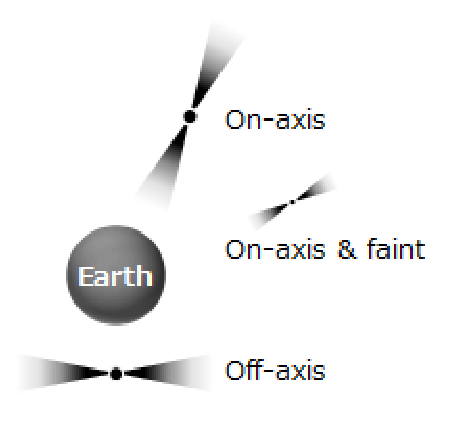
\includegraphics[width=3.5cm,clip]{transients/transients.GRB-afterglow.eps}
\end{wraptable}
GRBのガンマ線放射は高い指向性があり、その軸方向のみにガンマ線を放射するため、放射軸上に地球がなければガンマ線は観測されない。
一方でそれに付随する残光は指向性が高くないため、地球では残光のみが観測される、という状況を考えることができる \citep{1997ApJ...487L...1R}。
このような残光は親なし残光 (orphan afterglow) と呼ばれ、対応天体の見つからない電波トランジェントとして観測されうる\footnote{ガンマ線放射の軸が地球に向いていることを on-axis、向いていないことを off-axis と呼び、orphan afterglow は off-axis GRB afterglow と言い換えることができる。}。
\citet{2001ApJ...562L..55F}の見積もりによれば、99\% 以上のGRBで放射軸が地球から外れておりorphan afterglow のみが観測されると考えられるものの、従来の観測では候補天体が数例報告されているだけで、確定には至っていない。
SKAの広視野・高感度サーベイによって orphan afterglow を発見することができれば、GRB の物理の解明は大きく前進すると期待できる。
%

%
